
\tikzset{every picture/.style={line width=0.75pt}} %set default line width to 0.75pt        

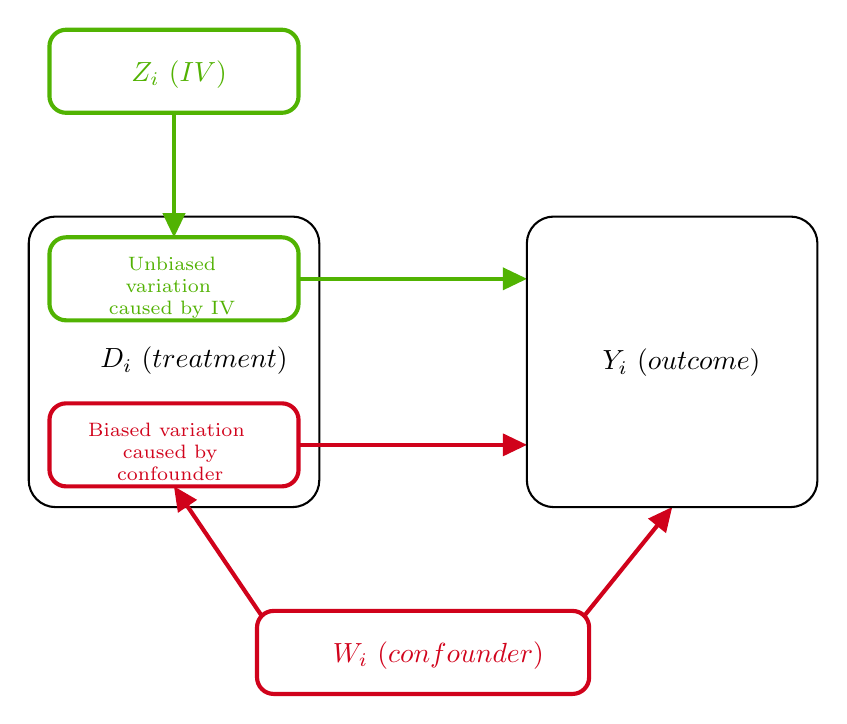
\begin{tikzpicture}[x=0.75pt,y=0.75pt,yscale=-1,xscale=1]
%uncomment if require: \path (0,524); %set diagram left start at 0, and has height of 524

%Rounded Rect [id:dp6497612275953306] 
\draw   (110,203) .. controls (110,195.82) and (115.82,190) .. (123,190) -- (237,190) .. controls (244.18,190) and (250,195.82) .. (250,203) -- (250,317) .. controls (250,324.18) and (244.18,330) .. (237,330) -- (123,330) .. controls (115.82,330) and (110,324.18) .. (110,317) -- cycle ;

%Rounded Rect [id:dp8673780682403747] 
\draw  [color={rgb, 255:red, 81; green, 179; blue, 2 }  ,draw opacity=1 ][line width=1.5]  (120,108) .. controls (120,103.58) and (123.58,100) .. (128,100) -- (232,100) .. controls (236.42,100) and (240,103.58) .. (240,108) -- (240,132) .. controls (240,136.42) and (236.42,140) .. (232,140) -- (128,140) .. controls (123.58,140) and (120,136.42) .. (120,132) -- cycle ;

%Straight Lines [id:da16218237230483512] 
\draw [color={rgb, 255:red, 208; green, 2; blue, 27 }  ,draw opacity=1 ][line width=1.5]    (240,300) -- (346,300) ;
\draw [shift={(350,300)}, rotate = 180] [fill={rgb, 255:red, 208; green, 2; blue, 27 }  ,fill opacity=1 ][line width=0.08]  [draw opacity=0] (11.61,-5.58) -- (0,0) -- (11.61,5.58) -- cycle    ;
%Straight Lines [id:da880895933850384] 
\draw [color={rgb, 255:red, 81; green, 179; blue, 2 }  ,draw opacity=1 ][line width=1.5]    (180,140) -- (180,196) ;
\draw [shift={(180,200)}, rotate = 270] [fill={rgb, 255:red, 81; green, 179; blue, 2 }  ,fill opacity=1 ][line width=0.08]  [draw opacity=0] (11.61,-5.58) -- (0,0) -- (11.61,5.58) -- cycle    ;
%Straight Lines [id:da6515543213351532] 
\draw [color={rgb, 255:red, 81; green, 179; blue, 2 }  ,draw opacity=1 ][line width=1.5]    (240,220) -- (346,220) ;
\draw [shift={(350,220)}, rotate = 180] [fill={rgb, 255:red, 81; green, 179; blue, 2 }  ,fill opacity=1 ][line width=0.08]  [draw opacity=0] (11.61,-5.58) -- (0,0) -- (11.61,5.58) -- cycle    ;
%Rounded Rect [id:dp3607596248065986] 
\draw  [color={rgb, 255:red, 208; green, 2; blue, 27 }  ,draw opacity=1 ][line width=1.5]  (220,388) .. controls (220,383.58) and (223.58,380) .. (228,380) -- (372,380) .. controls (376.42,380) and (380,383.58) .. (380,388) -- (380,412) .. controls (380,416.42) and (376.42,420) .. (372,420) -- (228,420) .. controls (223.58,420) and (220,416.42) .. (220,412) -- cycle ;

%Straight Lines [id:da11780334258026348] 
\draw [color={rgb, 255:red, 208; green, 2; blue, 27 }  ,draw opacity=1 ][line width=1.5]    (222,382) -- (182.24,323.31) ;
\draw [shift={(180,320)}, rotate = 55.89] [fill={rgb, 255:red, 208; green, 2; blue, 27 }  ,fill opacity=1 ][line width=0.08]  [draw opacity=0] (11.61,-5.58) -- (0,0) -- (11.61,5.58) -- cycle    ;
%Straight Lines [id:da6916433454902036] 
\draw [color={rgb, 255:red, 208; green, 2; blue, 27 }  ,draw opacity=1 ][line width=1.5]    (378,382) -- (417.49,333.11) ;
\draw [shift={(420,330)}, rotate = 128.93] [fill={rgb, 255:red, 208; green, 2; blue, 27 }  ,fill opacity=1 ][line width=0.08]  [draw opacity=0] (11.61,-5.58) -- (0,0) -- (11.61,5.58) -- cycle    ;
%Rounded Rect [id:dp8490775320395935] 
\draw  [color={rgb, 255:red, 208; green, 2; blue, 27 }  ,draw opacity=1 ][line width=1.5]  (120,288) .. controls (120,283.58) and (123.58,280) .. (128,280) -- (232,280) .. controls (236.42,280) and (240,283.58) .. (240,288) -- (240,312) .. controls (240,316.42) and (236.42,320) .. (232,320) -- (128,320) .. controls (123.58,320) and (120,316.42) .. (120,312) -- cycle ;

%Rounded Rect [id:dp9976354424664228] 
\draw   (350,203) .. controls (350,195.82) and (355.82,190) .. (363,190) -- (477,190) .. controls (484.18,190) and (490,195.82) .. (490,203) -- (490,317) .. controls (490,324.18) and (484.18,330) .. (477,330) -- (363,330) .. controls (355.82,330) and (350,324.18) .. (350,317) -- cycle ;

%Rounded Rect [id:dp7868826959222632] 
\draw  [color={rgb, 255:red, 81; green, 179; blue, 2 }  ,draw opacity=1 ][line width=1.5]  (120,208) .. controls (120,203.58) and (123.58,200) .. (128,200) -- (232,200) .. controls (236.42,200) and (240,203.58) .. (240,208) -- (240,232) .. controls (240,236.42) and (236.42,240) .. (232,240) -- (128,240) .. controls (123.58,240) and (120,236.42) .. (120,232) -- cycle ;


% Text Node
\draw (135,208) node [anchor=north west][inner sep=0.75pt]  [font=\scriptsize] [align=left] {\begin{minipage}[lt]{63.85pt}\setlength\topsep{0pt}
\begin{center}
\textcolor[rgb]{0.32,0.7,0.01}{Unbiased variation }\\\textcolor[rgb]{0.32,0.7,0.01}{caused by IV}
\end{center}

\end{minipage}};
% Text Node
\draw (128,288) node [anchor=north west][inner sep=0.75pt]  [font=\scriptsize] [align=left] {\begin{minipage}[lt]{72.98pt}\setlength\topsep{0pt}
\begin{center}
\textcolor[rgb]{0.82,0.01,0.11}{Biased variation }\\\textcolor[rgb]{0.82,0.01,0.11}{caused by confounder}
\end{center}

\end{minipage}};
% Text Node
\draw (158,113.4) node [anchor=north west][inner sep=0.75pt]    {$\textcolor[rgb]{0.32,0.7,0.01}{Z_{i} \ \text{(IV)}}$};
% Text Node
\draw (255,393.4) node [anchor=north west][inner sep=0.75pt]    {$\textcolor[rgb]{0.82,0.01,0.11}{W_{i} \ \text{(confounder)}}$};
% Text Node
\draw (385,252.4) node [anchor=north west][inner sep=0.75pt]    {$Y_{i} \ \text{(outcome)}$};
% Text Node
\draw (143,251.4) node [anchor=north west][inner sep=0.75pt]    {$D_{i} \ \text{(treatment)}$};


\end{tikzpicture}